%  Clam AntiVirus Bytecode Compiler: Internals Manual
%
%  Copyright (C) 2009 Sourcefire, Inc.
%  Author: Török Edvin <edwin@clamav.net>
%
%  This program is free software; you can redistribute it and/or modify
%  it under the terms of the GNU General Public License as published by
%  the Free Software Foundation; either version 2 of the License, or
%  (at your option) any later version.
%
%  This program is distributed in the hope that it will be useful,
%  but WITHOUT ANY WARRANTY; without even the implied warranty of
%  MERCHANTABILITY or FITNESS FOR A PARTICULAR PURPOSE.  See the
%  GNU General Public License for more details.
%
%  You should have received a copy of the GNU General Public License
%  along with this program; if not, write to the Free Software
%  Foundation, Inc., 51 Franklin Street, Fifth Floor, Boston,
%  MA 02110-1301, USA.

\documentclass[a4paper,titlepage,12pt,english]{book}
\usepackage{geometry}
\usepackage{pslatex}
\usepackage{fancyhdr}
\usepackage{longtable}
\usepackage{afterpage}
\usepackage{ifthen}
\usepackage{ifpdf}
\usepackage{titlesec}
\usepackage{microtype}
\usepackage[footnotesize,bf,justification=centering]{caption}
%%% general setup
\usepackage[english]{babel}
\usepackage[utf8x]{inputenc}
\usepackage[usenames, dvipsnames]{color}
\usepackage[perpage]{footmisc}
\usepackage{nomencl}
\usepackage{boxedminipage}
\usepackage{float}
\usepackage{algorithmic}
\usepackage{subfig}
\usepackage{moreverb}
\usepackage{listings}
\usepackage{prettyref}
\usepackage{varioref}
\lstset{language=C}
\lstset{escapeinside={(*@}{@*)}}
\lstset{numbers=left, numberstyle=\tiny, stepnumber=2,numbersep=5pt}
%\newrefformat{alg}{Algorithm \vref{#1}}
%\newrefformat{prg}{Program \vref{#1}}
%\newrefformat{fig}{Figure \vref{#1}}
%\newrefformat{tbl}{Table \vref{#1}}
\definecolor{LinkColor1}{rgb}{0.208,0.374,0.486}
\definecolor{LinkColor2}{rgb}{0.216,0.439,0.388}
\ifpdf
% pdfLaTeX setup
    \usepackage[pdftex]{graphicx}
    \DeclareGraphicsExtensions{.pdf}   %%% standard extension for included graphics
    \pdfcompresslevel=9
    \usepackage[pdftex,                %%% hyper-references for pdflatex
    bookmarks=true,%                   %%% generate bookmarks ...
    bookmarksnumbered=true,%           %%% ... with numbers
    bookmarksopen = true,
    breaklinks=true,%                  %%% break links if exceeding a single line
    citecolor=red,
    anchorcolor=green,
    colorlinks=true,
    hyperindex=true,
    hyperfigures,
    linkcolor=LinkColor1,
    filecolor=LinkColor2,
    menucolor=LinkColor2,
    urlcolor=LinkColor2,
    citecolor=LinkColor1,
    linktocpage,
    pagebackref,
    pdfpagelabels,
    pdfpagelayout=SinglePage,
    plainpages=false,
    hypertexnames=true,%              %%% needed for correct links to figures !!!
    linkbordercolor={0 0 1},           %%% blue frames around links
    pdfborder={0 0 0}]{hyperref}%      %%% pdfborder={0 0 1} is the default
    \hypersetup{
	pdfauthor = {T\"{o}r\"{o}k Edvin <edwin@clamav.net>},
	pdftitle =  {ClamAV Bytecode Compiler},
	pdfsubject = {Internals Manual},
	pdfkeywords = {}
    }
    \pdfadjustspacing=1                %%% force LaTeX-like character spacing
\else
    \usepackage{graphicx}
    \DeclareGraphicsExtensions{.eps,.ps}
    \usepackage{epsfig}
    \usepackage[ dvips,
                 bookmarks,
                 bookmarksopen = true,
                 bookmarksnumbered = true,
                 breaklinks = true,
                 linktocpage,
                 pagebackref,
                 colorlinks = false,
                 hyperindex = true,
                 hyperfigures
                 ]{hyperref}

\fi
%\usepackage{fancyvrb}
\usepackage{tikz}
%\usepackage{pgfplots}
\usepackage{framed}
%TODO: remove draft!
\usepackage{draftwatermark}

\usepackage[chapter]{algorithm}

%A4 settings
\ifpdf
   \pdfpageheight=297mm
   \pdfpagewidth=210mm
\else
   \setlength{\paperheight}{297mm}
   \setlength{\paperwidth}{210mm}
\fi
\makeglossary


\floatstyle{ruled}
\newfloat{program}{thp}{lop}
\floatname{program}{Program}

\definecolor{grey1}{gray}{0.8}
\definecolor{grey2}{gray}{0.3}
\definecolor{grey3}{gray}{0.6}
\definecolor{TitleColor}{rgb}{0.208,0.374,0.486}
\definecolor{NameColor}{rgb}{0.126,0.263,0.361}
\newlength{\grlength}
\setlength{\grlength}{\textwidth}
\addtolength{\grlength}{-9mm}
% Based on Antonina Liedtke's article in Linux+ 6/2003
\def\greyp{%
    \unitlength=1mm%
    \begin{picture}(0,0)
	\put(0,-1.5){\textcolor{grey1}{\rule{\grlength}{5.3mm}}\textcolor{grey2}%
	{\rule{9mm}{5.3mm}}\hss}
    \end{picture}
}
\def\greypl{%
    \unitlength=1mm%
    \begin{picture}(0,0)
	\put(0,-1.5){\textcolor{grey2}{\rule{9mm}{5.3mm}}\textcolor{grey1}%
	{\rule{\grlength}{5.3mm}}\hss}
    \end{picture}
}
\fancyhead{}
\fancyfoot{}

\titlelabel{\thetitle.\hspace{1ex}}
\renewcommand{\bottomtitlespace}{3\baselineskip}

\titleformat{\chapter}[display]
{\normalfont\Large\bfseries\sffamily}%
{\textcolor{TitleColor}{\MakeUppercase%
{\chaptertitlename}\ \Huge\thechapter}%
}%
{0pt}{\Huge\bfseries\rmfamily\filright\textcolor{NameColor}}%
[\vspace{-13pt}{\textcolor{grey3}%
{\titlerule[3pt]}}]

\titleformat{\section}
{\normalfont\Large\bfseries\sffamily}%
{\textcolor{TitleColor}{\Large\thesection.}%
}{1ex}{\textcolor{NameColor}}
[\vspace{-13pt}{\textcolor{grey3}%
{\titlerule[1.5pt]}}]

\titleformat{\subsection}
{\normalfont\large\bfseries}%
{\textcolor{TitleColor}{\large\sffamily%
\thesubsection.}}{1ex}%
{\textcolor{NameColor}}
[\vspace{-10pt}{\textcolor{grey1}%
{\titlerule[1pt]}}]


\titlespacing*{\chapter}{0pt}{50pt}{20pt}
\titlespacing*{\section} {0pt}%
{22pt plus 6pt minus 9pt}{12pt plus %
4pt minus 8pt}
\titlespacing*{\subsection} {0pt}%
{12pt plus 6pt minus 7pt}{6pt plus %
4pt minus 5pt}


\renewcommand{\headrulewidth}{0pt}
\fancyhead[LE]{\greypl\textbf{\sffamily{{\textcolor{white}{\thepage}}}}}
\fancyhead[RE]{\footnotesize{\nouppercase{\rightmark~}}}
\fancyhead[LO]{\footnotesize{\greyp{\nouppercase{\leftmark}}}}
\fancyhead[RO]{\textbf{\sffamily{{\textcolor{white}{\thepage}}~}}}
\fancyfoot[C]{\thepage}
 
\fancypagestyle{plain}{ %
\fancyhf{} % remove everything
\renewcommand{\headrulewidth}{0pt} % remove lines as well
\renewcommand{\footrulewidth}{0pt}}

\advance\headheight by 5.3mm
\advance\headsep by -3mm
%%%%%%%%%%%%%%%%%%%%%%%%%%%%%%%%%%%%%%%%%%%%%%%%%%%%%%%%%%%%%
% BEGIN DOCUMENT
%%%%%%%%%%%%%%%%%%%%%%%%%%%%%%%%%%%%%%%%%%%%%%%%%%%%%%%%%%%%%
\title{ClamAV Bytecode Compiler - Internals Manual}
\author{T\"{o}r\"{o}k Edvin}
\begin{document}

\frontmatter
\maketitle
\date{}
\setcounter{page}{1}
\pagestyle{fancy}
\tableofcontents
\vspace{1.0cm}
\noindent
\begin{boxedminipage}[b]{\textwidth}
    ClamAV Bytecode Compiler - Internals Manual,\\
    \copyright \  2009 Sourcefire, Inc.\\
    Authors: T\"{o}r\"{o}k Edvin\\
    This document is distributed under the terms of the GNU General
    Public License v2.\\

    Clam AntiVirus is free software; you can redistribute it and/or modify
    it under the terms of the GNU General Public License as published by
    the Free Software Foundation; either version 2 of the License, or
    (at your option) any later version.\\

    This program is distributed in the hope that it will be useful,
    but WITHOUT ANY WARRANTY; without even the implied warranty of
    MERCHANTABILITY or FITNESS FOR A PARTICULAR PURPOSE.  See the
    GNU General Public License for more details.\\

    You should have received a copy of the GNU General Public License
    along with this program; if not, write to the Free Software
    Foundation, Inc., 51 Franklin Street, Fifth Floor, Boston,
    MA 02110-1301, USA.
\end{boxedminipage}

\vspace{0.3cm}
\noindent
\begin{boxedminipage}[b]{\textwidth}
    ClamAV and Clam AntiVirus are trademarks of Sourcefire, Inc.
\end{boxedminipage}

\mainmatter
\chapter{Overview}

This manual describes internals details about the bytecode API, compiler, and
libclamav bytecode interpreter/JIT.
This manual is only of interest to ClamAV developers, see the
"ClamAV Bytecode Compiler User Manual" on how to write bytecode signatures.

\chapter{Bytecode libclamav hooks}
\section{Logical Signature hooks}
\section{PE hooks}

\section{Adding a new hook}
A bytecode hook consists of the following:
\begin{itemize}
\item special global variables mapped to clamav internal structures,
\item bytecode invoked at certain points in libclamav
\item bytecode APIcalls specific to the hook
\end{itemize}

\subsection{Adding new special globals for hooks}
In the bytecode there are several special global variables named
\verb+__clambc_*+, which are mapped to libclamav internal variables.

These are globals from the bytecode's point of view to make bytecode writing
easier, but they are not real globals in libclamav (it wouldn't be threadsafe).
Instead in libclamav these "special globals" are stored in \verb+struct cli_bc_ctx.hooks+,
and the JIT/interpreter inserts special code to access fields of this struct as
if they were globals.

Steps to add a new global to the bytecode compiler:
\begin{itemize}
\item Choose a unique name for the global
(have a look at \verb+clang/lib/Headers/bytecode_api.h+)

\item Add a new value to \verb+enum bc_global+ in \verb+ClamBC/clambc.h+ named
\verb+GLOBAL_+ followed by the uppercase name of the global. Make sure you add a
new global before \verb+_LAST_GLOBAL+, and don't change the order of the other
enum values (this ensures that bytecodes that don't use the new global continue
to work properly on old versions of libclamav that don't have the new global).

\item Declare the global's name in \verb+ClamBC/ClamBCModule.cpp+: 
 
\verb+globalsMap["__clambc_<name>"] = GLOBAL_<NAME>;+ where \verb+<name>+
and \verb+<NAME>+ are the lowercase/uppercase names of the global.

\item Declare the new global in \verb+clang/lib/Headers/bytecode_api.h+, order
of declaration  of globals doesn't matter here. The global must be declared as
\verb+extern const+ and named \verb+__clambc_+ followed by the lowercase name of
the global.

\item Run \verb+./sync_clamav.sh+ to generate \verb+bytecode_api_decl.c.h+,
\verb+bytecode_api_impl.h+, \verb+bytecode_hooks.h+.
\end{itemize}

Steps to add a new global to libclamav (needed if you add to compiler):
\begin{itemize}
\item In \verb+libclamav/bytecode.c:cli_bytecode_context_alloc()+ initialize the
field of \verb+ctx->hooks+ corressponding to the new global
\item Set the field coresponding to the global in the struct \verb+ctx->hooks+
in one of the API hooks, or introduce a new API hook that sets it.
\item Note that the pointer set must be valid during the entire execution of the
bytecode.
\end{itemize}

\subsection{Adding new bytecode APIs}
Bytecode APIs are external function calls from the bytecode into special
entrypoints in libclamav.

To add a new API follow these steps:
\begin{itemize}
\item Add the prototype for the new API to
\verb+clang/lib/Headers/bytecode_api.h+, inside \verb+#ifdef __CLAMBC__+
\item Run \verb+./sync_clamav.sh+ to synchronize with libclamav
\item Implement the new \verb+cli_bcapi_+ in \verb+libclamav/bytecode_api.c+
\item You can store values in fields of \verb+ctx+, which is a hidden parameter,
    not accessible from bytecode.
\item You can introduce new fields in \verb+ctx+ if needed to implement the API
\item Do validation on input parameters, and any necessary security checks in
the implementation of the API
\item Create a new test in \verb+examples/in/+, with the extension \verb+.o1.c+,
    and update \verb+sync_clamav.sh+ to copy it to \verb+unit_tests/input+
\item Add a new testcase to \verb+unit_tests/check_bytecode.c+:
  \begin{itemize}
  \item Add a new \verb+test_+ function, and add it to the testcase with
  \verb+tcase_add_test+
  \item Call \verb+cl_init+ and \verb+runtest+ similar to other existing unit
  tests, but change the filename to the newly added unittest's name
  \item Run make check, make sure it passes
  \end{itemize}
\end{itemize}


\chapter{Updating LLVM}
\section{Update LLVM from upstream SVN}
% TODO: use git when LLVM will have official git mirror
\begin{itemize}
\item \verb+cd+ into the git-svn dir of upstream LLVM
\item Update LLVM \footnote{this may require updating the svn-authors file}:
\begin{verbatim}
$ cd llvm
$ git svn fetch
$ git svn rebase --local
\end{verbatim}
\item Update clang:
\begin{verbatim}
$ cd clang
$ git svn fetch
$ git svn rebase --local
\end{verbatim}
\item Build it:
\begin{verbatim}
$ cd ../obj && ../llvm/configure --enable-optimized
$ make -j8
\end{verbatim}
\item All tests must pass before merging to clamav: \verb+make check-all+
\item (Optional) Build ClamAV with clang/x86 backend to test that the C frontend
works:
\begin{verbatim}
$ cd /path/to/clamavsrc
$ ./configure CC=/path/to/clambc-compiler/obj/Release/bin/clang
$ make -j4
$ make check -j4
\end{verbatim}
\end{itemize}

\section{Merging LLVM to ClamAV bytecode compiler}
Use the \verb+merge-new.sh+ script in the bytecode compiler repository.
If there are no conflicts then the script takes care of merging, and comitting
and.

If there are conflicts, the script will stop, and output an error message about
the failed merge.

Fix the conflicts by using \verb+git mergetool+, then
commit the result using \verb+git commit+.

Note that if llvm merge failed, clang is not merged either, so you should resume
the merge of clang (easiest is to just rerun the script).

Then run \verb+make check-all+ for the compiler too.

Note: the script is now doing normal merges (i.e. unsquashed), to visualize just
"our" history use git log --first-parent

\section{Merging LLVM to ClamAV (libclamav)}
Update llvm remote: \verb+git remote update llvm-upstream+.

Use the script \verb|libclamav/c++/merge.sh| as above, from root of ClamAV
source directory, there will be delete/modify conflicts.

Next run the script \verb|libclamav/c++/strip-llvm.sh|, from the
\verb|libclamav/c++| directory, and see if there are any
unneeded dirs left in LLVM. If there are, update the strip script, and rerun it.
Now resolve any merge conflicts, commit the merge, and tag it as instructed by
merge.sh.

Regenerate configure with autoconf 2.65:
\begin{itemize}
\item \verb+cd llvm/autoconf+
\item \verb+sed -i '/Your/d' AutoRegen.sh+
\item \verb+./AutoRegen.sh+
\item \verb+git checkout AutoRegen.sh+
\item \verb+cd ..; git add configure; git add include/llvm/Config/config.h.in+
\end{itemize}

After the merge is complete, update the build files (if needed):
\begin{itemize}
\item do a Debug build of upstream LLVM
\item Run \verb|libclamav/c++/GenList.pl /path/to/llvm-objdir >out|
\item Copy the \_SOURCES definitions from \verb+out+ to
\verb|libclamav/c++/Makefile.am|
\item Run automake in \verb|libclamav/c++|
\item Update the autogenerated files
\item Build ClamAV
\item Update to latest LLVM API (if needed)
\item Build ClamAV
\item Update win32 proj files: \verb+win32/update-win32.pl --regen+
\end{itemize}

To update the autogenerated files:
\begin{itemize}
\item Configure ClamAV in maintainer mode
\footnote{Note that this must be a srcdir == objdir build}:\\
\verb|./configure --enable-maintainer-mode|
\item Build it:\\
\verb|make -j8|
\item If tblgen fails to build, review the list of files in
\verb+tblgen_SOURCES+
\item Review what files changed files (probably .inc and .gen files):\\
\verb|git status|
\item Commit the result:\\
\verb|git commit -a -m "Update autogenerated files after LLVM import"|
\item Fully clean the build dir
\footnote{Be careful to run this inside the ClamAV source dir, and not some other git repository}:\\
\verb|git clean -xfd|
\item Test a normal (non-maintainer build, can be objdir != srcdir):\\
\verb|./configure && make && make check|
\end{itemize}

Run \verb+make check+ from top-level builddir, this will run the LLVM tests too,
make sure all of them pass.

Build ClamAV with \verb+--enable-all-jit-targets+ to test that all supported JIT
targets build.

\chapter{ClamAV bytecode language}
The bytecode that ClamAV loads is a simplified form of the LLVM Intermediate Representation, and as such it is language-independent.

However currently the only supported language from which such bytecode can be
generated is a simplified form of C.

The ClamAV bytecode backend translates from LLVM IR to ClamAV bytecode.
Theoretically it could translate any LLVM IR which meets these constraints:
\begin{itemize}
\item No external function calls, except those defined by the ClamAV API
\item No inline assembly
\item ...
 %TODO: the constraints
\end{itemize}

Thus (theoretically) any language that doesn't need an external language runtime (or
the runtime can be compiled to the above restricted set of LLVM IR), could be
compiled to ClamAV bytecode.

There are currently no plans currently to support any other language than C (maybe C++ when
clang will support it).

\section{Predefines}
The following macros are predefined:
\lstset{basicstyle=\tiny}
\lstinputlisting{predefines}
\lstset{basicstyle=\footnotesize}

\section{ClamAV API header restrictions}
The ClamAV API header file (\verb+bytecode_api.h+, and any files included by it) must be both valid C code, and conform to the following BNF grammar:
%TODO: write the grammar here

The reason is that the \verb+ifacegen+ program must be able to parse it to
generate the api description, and glue code, and it only recognizes the above
BNF grammar.

This also adds portability checks: any code conforming to that grammar should
work properly both in the interpret and the JIT, even though a number of things
have changed (such as sizeof int, which is why only fixed-size integers are
allowed in the API).
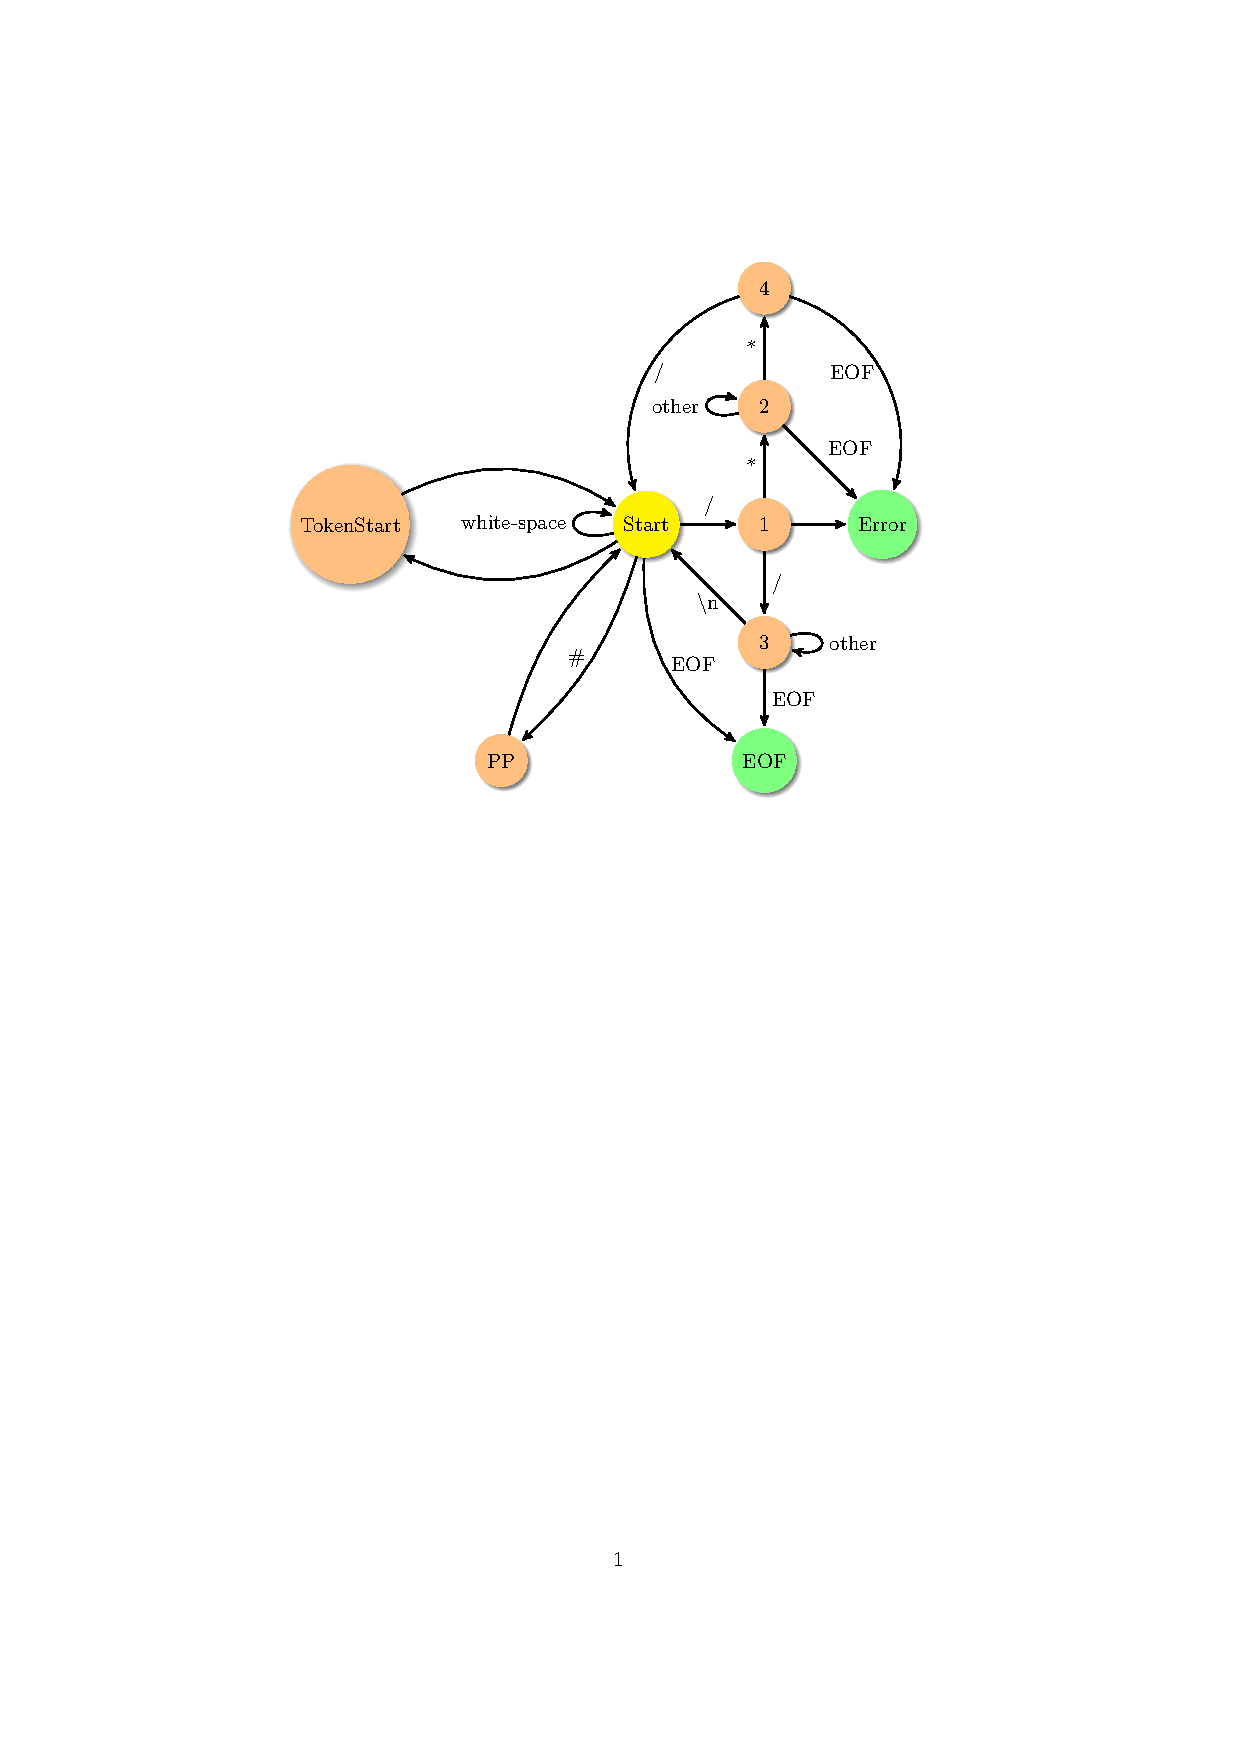
\includegraphics{ifacegen-automata.pdf}
%
%\begin{grammar}
%[(colon){ ::$\Rightarrow$ }]
%[(semicolon){ $|$}]
%[(comma){}]
%[(period){\\}]
%[(quote){\begin{bf}}{\end{bf}}]
%[(nonterminal){$\langle$}{$\rangle$}]
%<API header> : $\epsilon$; <declaration>, <API header>.
%<declaration>: <type spec>, <function or struct decl>.
%<function or struct decl>: identifier, <function declaration>; "\{", <struct declaration>.
%<expression>:<number>;\\
%<number>, <relational operator>, <number>.
%<number>:<digit>;<digit>,<number>.
%<digit>:"0";"1";"2";"3";"4";"5";"6";"7";"8";"9".
%<relational operator>:"$=$";"$\lessthan\greaterthan$";
%"$\lessthan$";"$\greaterthan$";
%"$\lessthan=$";"$\greaterthan=$";"in".
%\end{grammar}


\chapter{Publishing ClamAV bytecode}
\section{Pre-publish tests}

The following tests are automatically performed prepublish:
%TODO: this will have to be implemented on the SI
\begin{itemize}
 \item Compile the source code using the latest version of the ClamAV bytecode compiler (with user-specified optimization level):
\begin{verbatim}
$ clambc-compiler bytecode-726914.c -o testdir/bytecode-726914.cbc -O<N>
\end{verbatim}
 \item Try to load the bytecode using the latest 2 stable version of ClamAV, both in JIT and interpreter mode
\footnote{Since there is no stable version supporting bytecode, and the bytecode will be distributed in a separate cvd,
for now we should test with latest nightly snapshot of ClamAV-devel. 
For 0.97 we should test with: 0.97, 0.96.1 (assuming those are latest 2 versions)}
\begin{verbatim}
$ export STABLEBIN=/usr/local/clamav-stable/bin
$ export DEVBIN=/usr/local/clamav-devel/bin
$ $STABLEBIN/clamscan -dtestdir/ -r /path/to/clamav-testfiles/
$ $DEVBIN/clamscan -dtestdir/ -r /path/to/clamav-testfiles/
$ $STABLEBIN/clamscan --force-interpreter -dtestdir/\
 -r /path/to/clamav-testfiles/
$ $DEVBIN/clamscan --force-interpreter -dtestdir/\
 -r /path/to/clamav-testfiles/
\end{verbatim}
 \item Scan the sample(s) that will have this bytecode associated with the bytecode loaded (both interpreter and JIT mode):
 \item Scan the FPfarm
\begin{verbatim}
$ $STABLEBIN/clamscan -dtestdir/ -r /path/to/fpfarm/
$ $DEVBIN/clamscan -dtestdir/ -r /path/to/fpfarm/
\end{verbatim}
\end{itemize}

\section{Building bytecode.cvd}
Sigtool will perform some minimal checks on the bytecode prior to creating CVD:
\begin{itemize}
\item writes its own version in the header
\item load the bytecode using libclamav API
\item check that the interpreter and JIT can load it
\item check that it is compilable to all configured targets (x86, ppc at least)
\item check that the bytecode is production version (no debug metadata, all
header fields are filled out, has associated virusname)
\end{itemize}
\begin{verbatim}
%TODO: sigtool commandline
\end{verbatim}

\chapter{Copyright}

The ClamAV Bytecode Compiler is released under the GNU General Public License
version 2.

The following directories are under the GNU General Public License version 2:
libclambcc, docs, clambcc, test, examples, clambc-ifacegen, headers.

{\footnotesize
\begin{verbatim}
Copyright (C) 2009 Sourcefire, Inc.

This program is free software; you can redistribute it and/or modify
it under the terms of the GNU General Public License version 2 as
published by the Free Software Foundation.

This program is distributed in the hope that it will be useful,
but WITHOUT ANY WARRANTY; without even the implied warranty of
MERCHANTABILITY or FITNESS FOR A PARTICULAR PURPOSE.  See the
GNU General Public License for more details.

You should have received a copy of the GNU General Public License
along with this program; if not, write to the Free Software
Foundation, Inc., 51 Franklin Street, Fifth Floor, Boston,
MA 02110-1301, USA.
\end{verbatim}
}

It uses the LLVM compiler framework, contained in the following directories:
llvm, clang. They have this copyright:
{\footnotesize
\begin{verbatim}
==============================================================================
LLVM Release License
==============================================================================
University of Illinois/NCSA
Open Source License

Copyright (c) 2003-2009 University of Illinois at Urbana-Champaign.
All rights reserved.

Developed by:

    LLVM Team

    University of Illinois at Urbana-Champaign

    http://llvm.org

Permission is hereby granted, free of charge, to any person obtaining a copy of
this software and associated documentation files (the "Software"), to deal with
the Software without restriction, including without limitation the rights to
use, copy, modify, merge, publish, distribute, sublicense, and/or sell copies
of the Software, and to permit persons to whom the Software is furnished to do
so, subject to the following conditions:

    * Redistributions of source code must retain the above copyright notice,
      this list of conditions and the following disclaimers.

    * Redistributions in binary form must reproduce the above copyright notice,
      this list of conditions and the following disclaimers in the
      documentation and/or other materials provided with the distribution.

    * Neither the names of the LLVM Team, University of Illinois at
      Urbana-Champaign, nor the names of its contributors may be used to
      endorse or promote products derived from this Software without specific
      prior written permission.

THE SOFTWARE IS PROVIDED "AS IS", WITHOUT WARRANTY OF ANY KIND, EXPRESS OR
IMPLIED, INCLUDING BUT NOT LIMITED TO THE WARRANTIES OF MERCHANTABILITY, FITNESS
FOR A PARTICULAR PURPOSE AND NONINFRINGEMENT.  IN NO EVENT SHALL THE
CONTRIBUTORS OR COPYRIGHT HOLDERS BE LIABLE FOR ANY CLAIM, DAMAGES OR OTHER
LIABILITY, WHETHER IN AN ACTION OF CONTRACT, TORT OR OTHERWISE, ARISING FROM,
OUT OF OR IN CONNECTION WITH THE SOFTWARE OR THE USE OR OTHER DEALINGS WITH THE
SOFTWARE.

==============================================================================
Copyrights and Licenses for Third Party Software Distributed with LLVM:
==============================================================================
The LLVM software contains code written by third parties.  Such software will
have its own individual LICENSE.TXT file in the directory in which it appears.
This file will describe the copyrights, license, and restrictions which apply
to that code.

The disclaimer of warranty in the University of Illinois Open Source License
applies to all code in the LLVM Distribution, and nothing in any of the
other licenses gives permission to use the names of the LLVM Team or the
University of Illinois to endorse or promote products derived from this
Software.

The following pieces of software have additional or alternate copyrights,
licenses, and/or restrictions:

Program             Directory
-------             ---------
Autoconf            llvm/autoconf
                    llvm/projects/ModuleMaker/autoconf
                    llvm/projects/sample/autoconf
CellSPU backend     llvm/lib/Target/CellSPU/README.txt
Google Test         llvm/utils/unittest/googletest
OpenBSD regex       llvm/lib/Support/{reg*, COPYRIGHT.regex}
\end{verbatim}
}


\end{document}
